\documentclass[9pt,twoside]{pnas-new}
% Use the lineno option to display guide line numbers if required.

\articletype{Social Sciences}%%%% Article topic/classification

\templatetype{pnasmathematics} % Choose template
% {pnasresearcharticle} = Template for a two-column research article
% {pnasmathematics} = Template for a one-column mathematics article
% {pnasinvited} = Template for a PNAS invited submission
%\onecolumn

\usepackage{booktabs}

\begin{document}

\title{Where the neurologists are not: measuring the gap between neurological disease burden and the capacity to treat it}

% Use letters for affiliations, numbers to show equal authorship (if applicable) and to indicate the corresponding author
\author[a,1]{Alanna Polyak}

\affil[a]{Department of Quantitative Social Science, Dartmouth College, Hanover, NH 03755}

% Please give the surname of the lead author for the running footer
\leadauthor{Polyak}

% Please add a significance statement to explain the relevance of your work
\significancestatement{Specialists per country is the statistic normally used to describe where medical capacity sits, and it answers the wrong question. Combining three World Health Organization sources across 52 countries, this study shows that the countries holding the largest share of the world's stroke burden hold the smallest share of its neurologists, by a factor of roughly thirty-four. It then shows that national counts overstate what most residents can reach, because the poorer a country is, the more completely its specialists concentrate in the capital. In low-income countries the specialist density facing a rural resident is not merely low but exactly zero, which makes the usual language of ratios inapplicable.}

% Please include corresponding author, author contribution and author declaration information
\authorcontributions{A.P. designed the study, wrote all analysis code, performed the analysis, and wrote the paper.}
\authordeclaration{The author declares no competing interests.}
\correspondingauthor{\textsuperscript{1}To whom correspondence should be addressed. E-mail: alanna.g.polyak.28\@dartmouth.edu}

% At least three keywords are required at submission. Please provide three to five keywords, separated by the pipe symbol.
\keywords{health workforce $|$ neurological disease $|$ global health equity $|$ rural access $|$ inequality measurement}

\begin{abstract}
Neurological disease burden and the workforce trained to treat it are not distributed alike. Combining the WHO/WFN Neurology Atlas, the WHO Global Dementia Observatory and WHO Global Health Estimates across 52 countries, I measure that mismatch three ways. First, a scale-free burden-to-capacity share ratio places the median low- or middle-income country at 13.1, meaning it carries thirteen times as large a share of the sample's stroke burden as of its neurologists, against 0.38 for the median high-income country: a factor of 34. Two countries report zero neurologists and cannot be placed on the scale at all. Second, capacity is distributed across countries with a Gini coefficient of 0.61 (95\% bootstrap CI 0.43--0.73), the poorer half of countries holding 6\% of the sampled workforce. Third, national density overstates access wherever specialists remain urban: an Urban Concentration Index falls from 0.95 in low-income countries to 0.52 in high-income ones, and the effective density facing a rural resident of a low-income country is exactly zero, because no low-income country in the Atlas reports a neurologist practicing rurally. Because country-level regressions on 19 to 35 observations are underpowered, all inference is conducted on binned groups. A bounding exercise shows burden would have to be overstated by a factor of 34 in low- and middle-income countries for the central result to reverse. All analysis is descriptive; no causal effect is estimated.
\end{abstract}

\dates{This manuscript was compiled on \today}
\doi{\url{www.pnas.org/cgi/doi/10.1073/pnas.XXXXXXXXXX}}

\maketitle
\thispagestyle{firststyle}
\ifthenelse{\boolean{shortarticle}}{\ifthenelse{\boolean{singlecolumn}}{\abscontentformatted}{\abscontent}}{}


\Firstpage

%The \Firstpage command is used to format the first page text column size. The same size will be maintained for subsequent paragraph until the \Endparasplit or \Parasplit command is encountered.


% If your first paragraph (i.e. with the \dropcap) contains a list environment (quote, quotation, theorem, definition, enumerate, itemize...), the line after the list may have some extra indentation. If this is the case, add \parshape=0 to the end of the list environment.
\dropcap{N}eurological disorders are among the largest contributors to global
disability, and the workforce able to diagnose and manage them is among the most
unevenly distributed of any medical specialty. This paper asks a distributional
question: are the countries carrying the heaviest neurological disease burden
the ones with the capacity to treat it?

% Note: please start your introduction without including the word ``Introduction'' as a section heading (except for math articles in the Physical Sciences section); this heading is implied in the first paragraphs.

\subsection*{Related work}

The question is not new, and this is not the first analysis of neurological
workforce scarcity. The WHO and World Federation of Neurology Atlas has
documented that scarcity across two editions and established that resources are
severely limited in low-income countries \cite{atlas2017}. Prior work has also
established that specialist supply is concentrated in high-income settings and
that rural residents face additional access barriers.

What the Atlas does not do, and what this analysis adds, is link capacity to
\emph{need}. The Atlas reports medians within income groups and WHO regions,
presents no country-level workforce estimates, and includes no burden measure at
all. It can therefore say that low-income countries have fewer neurologists, but
not whether the countries with the least capacity are the ones carrying the
heaviest burden, which is the question that matters for priority-setting.
Grouped medians also suppress within-group variation entirely, so a low-income
country with functioning services and one with none are indistinguishable in the
published tables. This paper extends that literature in three ways: it joins
capacity to a burden measure at the country level, it reports a distributional
statistic rather than a central tendency, and it separates how much capacity
exists from where inside a country that capacity sits.\Endparasplit

%The \Endparasplit command is used to end the formatting of the text column size that was set by the \Firstpage command. This will restore the default column size for the subsequent text.
%
%The \Parasplit command should be used if the page ends in the middle of a paragraph, allowing the column formatting to continue seamlessly on the next page.

\section*{Data}

\paragraph{Sources.} Three WHO products and one survey inventory are used.
(i) The \emph{Global Dementia Observatory} indicator \texttt{GDO\_q6x1\_2} gives
neurologists per 100{,}000 population, self-reported by ministries of health.
(ii) GDO indicator \texttt{GDO\_q8x3\_1} gives the furthest geographic level at
which dementia diagnostic services are available, on an ordered three-level
scale. (iii) WHO \emph{Global Health Estimates} series
\texttt{SA\_0000001689} gives age-standardized stroke DALYs per 100{,}000.
(iv) The WHO/WFN \emph{Neurology Atlas}, second edition, supplies the country to
WHO-region to World-Bank-income-group crosswalk from Annex 1 and the aggregate
workforce gradients from Tables 2--3 and Figures 11, 12 and 16. A DHS survey
inventory is used only to describe coverage for a possible subnational
extension.

\paragraph{Time window.} Capacity and service reach are 2017, the fielding year
of the second Atlas and the GDO round used. Burden is \textbf{2004}, which is
the only round of the WHO stroke DALY series exposed by the GHO API at the time
of writing. The thirteen-year offset is the single largest weakness in the
analysis and is the reason RQ1 is framed as describing a gap rather than
estimating one.

\paragraph{Unit of analysis.} In the original sources the unit differs by
product: GDO records are one row per country per indicator per round; GHE records
are one row per country per cause per age-standardization per year; the Atlas
Annex is one row per responding Member State. The unit of analysis
\emph{used here} is the \textbf{country}. Every source is collapsed to one row
per ISO3 code before merging, and no country appears twice.

\paragraph{Missingness in key fields.} The panel has 52 countries.
Neurologist density is missing for \textbf{33 of 52} (63\%), service reach for
5 (10\%), income group for 13 (25\%), and stroke burden for none. WHO encodes
absence as the strings ``Not available'', ``Not applicable'', ``No data'' and
``Not reported'' rather than as empty cells; these are converted to missing in
\texttt{code/03\_clean\_merge.py} (lines 19--20) before any numeric coercion, so
that a placeholder string cannot silently become a zero. Missingness is not
random: countries that report a workforce count plausibly have stronger health
information systems, which biases the sample toward better-resourced countries
and therefore \emph{understates} the true gap.

\paragraph{Limitations of the sources.} All WHO instruments here are ministry
questionnaires, self-reported and unaudited, with no full-time-equivalent
adjustment, so a neurologist working one clinic day a week counts the same as
one working five. Stroke stands in for neurological burden generally. Measured
burden itself depends on diagnostic capacity, which is the exposure of interest,
so the two are entangled by construction; this is addressed by bounding rather
than by adjustment.

\section*{Methods}

\paragraph{Cleaning.} \texttt{code/03\_clean\_merge.py} performs every cleaning
step. WHO placeholder strings are mapped to missing (line 20); the ordered
service-reach question is mapped from text to an integer scale via
\texttt{ACC\_SCALE} in \texttt{utils.py} (line 36); and two binary indicators are
derived from that scale, \texttt{beyond\_capital} for levels $\ge 2$ and
\texttt{reaches\_rural} for level $3$ (lines 42--43).

\paragraph{Merging.} Capacity and service reach are combined with an
\textbf{outer join on ISO3}, deliberately, so that a country reporting one but
not the other is retained rather than dropped; this yields 52 rows. Burden and
the Atlas crosswalk are then attached with \textbf{left joins on ISO3},
preserving those 52 rows. All matching is \textbf{exact on ISO3 country code},
not fuzzy on country name, which avoids the standard failure mode where
``Republic of Korea'' and ``Korea, Rep.'' fail to match. The script prints row
counts before and after every join, and the printed counts appear in
\texttt{output/log\_03\_clean\_merge.txt}.

\paragraph{Variable definitions.} The \textbf{burden-to-capacity share ratio}
for country $i$ is
%
\begin{align*}
R_i = \frac{b_i / \sum_j b_j}{c_i / \sum_j c_j} \numberthis \label{eqn:ratio}
\end{align*}
%
where $b_i$ is the age-standardized stroke DALY rate and $c_i$ is neurologist
density. Both terms are shares, so $R_i$ is invariant to the units of either
input. $R_i = 1$ means country $i$ holds exactly as large a share of the
sample's burden as of its workforce; $R_i = 13.1$ means the same staff are
stretched over thirteen times the need. It is undefined at $c_i = 0$, and those
countries are reported separately rather than dropped.

The \textbf{Urban Concentration Index} and \textbf{effective rural density} are
%
\begin{align*}
\mathrm{UCI}_g &= \frac{p^{\text{cap}}_g - p^{\text{rur}}_g}{100} \numberthis \label{eqn:uci} \\
D^{\text{eff}}_g &= m_g \cdot \frac{p^{\text{rur}}_g}{100} \numberthis \label{eqn:erd}
\end{align*}
%
where $p^{\text{cap}}_g$ and $p^{\text{rur}}_g$ are the percentages of countries
in income group $g$ reporting neurologists in the capital and in rural areas,
and $m_g$ is the group's median density. UCI is bounded $[0,1]$; a value of 1
means every country has capital coverage and none has rural coverage.
$D^{\text{eff}}_g$ rescales national density by the share of countries where a
rural resident could reach anyone at all.

Inequality is measured by the \textbf{Gini coefficient} of neurologist density,
computed by the sorted-index formula in \texttt{utils.py} (line 214) and
independently by trapezoidal integration under the Lorenz curve (line 233). The
two agree to $1.1\times10^{-16}$, which is a check on the implementation rather
than a result.

\paragraph{Inference, and why no country-level regression is reported.} This is
a \textbf{descriptive} analysis. There is no source of causal identification: no
randomization, no instrument, no policy discontinuity, and national income drives
both capacity and measured burden. No causal effect is estimated or implied.

With 19 to 35 observations, a fitted country-level slope would be badly
underpowered, so no slope is reported as a headline result. Countries are binned
by World Bank income group and the groups compared directly, with a Welch
$t$-test, a Mann-Whitney $U$, a 20{,}000-draw permutation test that assumes
nothing about distributional shape, a one-way ANOVA and Kruskal-Wallis across
three bins, a chi-square on the reach-by-income contingency table, and a
logistic regression of rural reach on high income. A regression \emph{is} fitted
in \texttt{code/07\_regression\_and\_interactions.py}, but only to demonstrate
two solvers agreeing (normal equations against gradient descent, to
$4.4\times10^{-16}$) and to test an interaction the sample cannot resolve.

\section*{Results}

\paragraph{The analysis sample.} Table~\ref{tab:sample} characterizes it. Of 52
countries in the merged panel, 19 support the RQ1 comparison and 35 the RQ3
comparison; the difference is entirely driven by which WHO indicators a country
chose to answer.

\begin{table}[t!]
\centering
\caption{The analysis sample. Row counts are after the merges described in
Methods; every source is 2017 except stroke burden, which is 2004. The two
analysis samples differ because reporting a workforce count and reporting a
service-reach level are separate questionnaire items, answered by overlapping
but non-identical sets of countries.}
\label{tab:sample}
\begin{tabular}{lr}
\toprule
Measure & $n$ \\
\midrule
Countries in merged panel & 52 \\
\quad with neurologist density (WHO GDO, 2017) & 19 \\
\quad with service-reach level (WHO GDO, 2017) & 47 \\
\quad with stroke DALY rate (WHO GHE, 2004) & 52 \\
\quad with World Bank income group (Atlas, 2017) & 39 \\
\midrule
RQ1 analysis sample: capacity and burden & 19 \\
RQ3 analysis sample: reach and income group & 35 \\
\bottomrule
\end{tabular}

\addtabletext{Countries reporting zero neurologists are retained in the panel but
cannot be placed on the ratio scale of Eq.~\ref{eqn:ratio}.}
\end{table}

\subsection*{Capacity is not aligned with burden}

On the share ratio, the median high-income country sits at \textbf{0.38} and the
median low- or middle-income country at \textbf{13.12}, a factor of
\textbf{34.3}. Myanmar reaches 69.7, Bangladesh 49.1, Togo 43.9. At the other
end Switzerland sits at 0.07. Eswatini and Fiji report \emph{zero} neurologists
and cannot be placed on the scale at all, while carrying stroke DALY rates of
1{,}536 and 994 per 100{,}000. Figure~\ref{fig:ratio} shows the full ordering.

\begin{figure}%[tbhp]
\centering
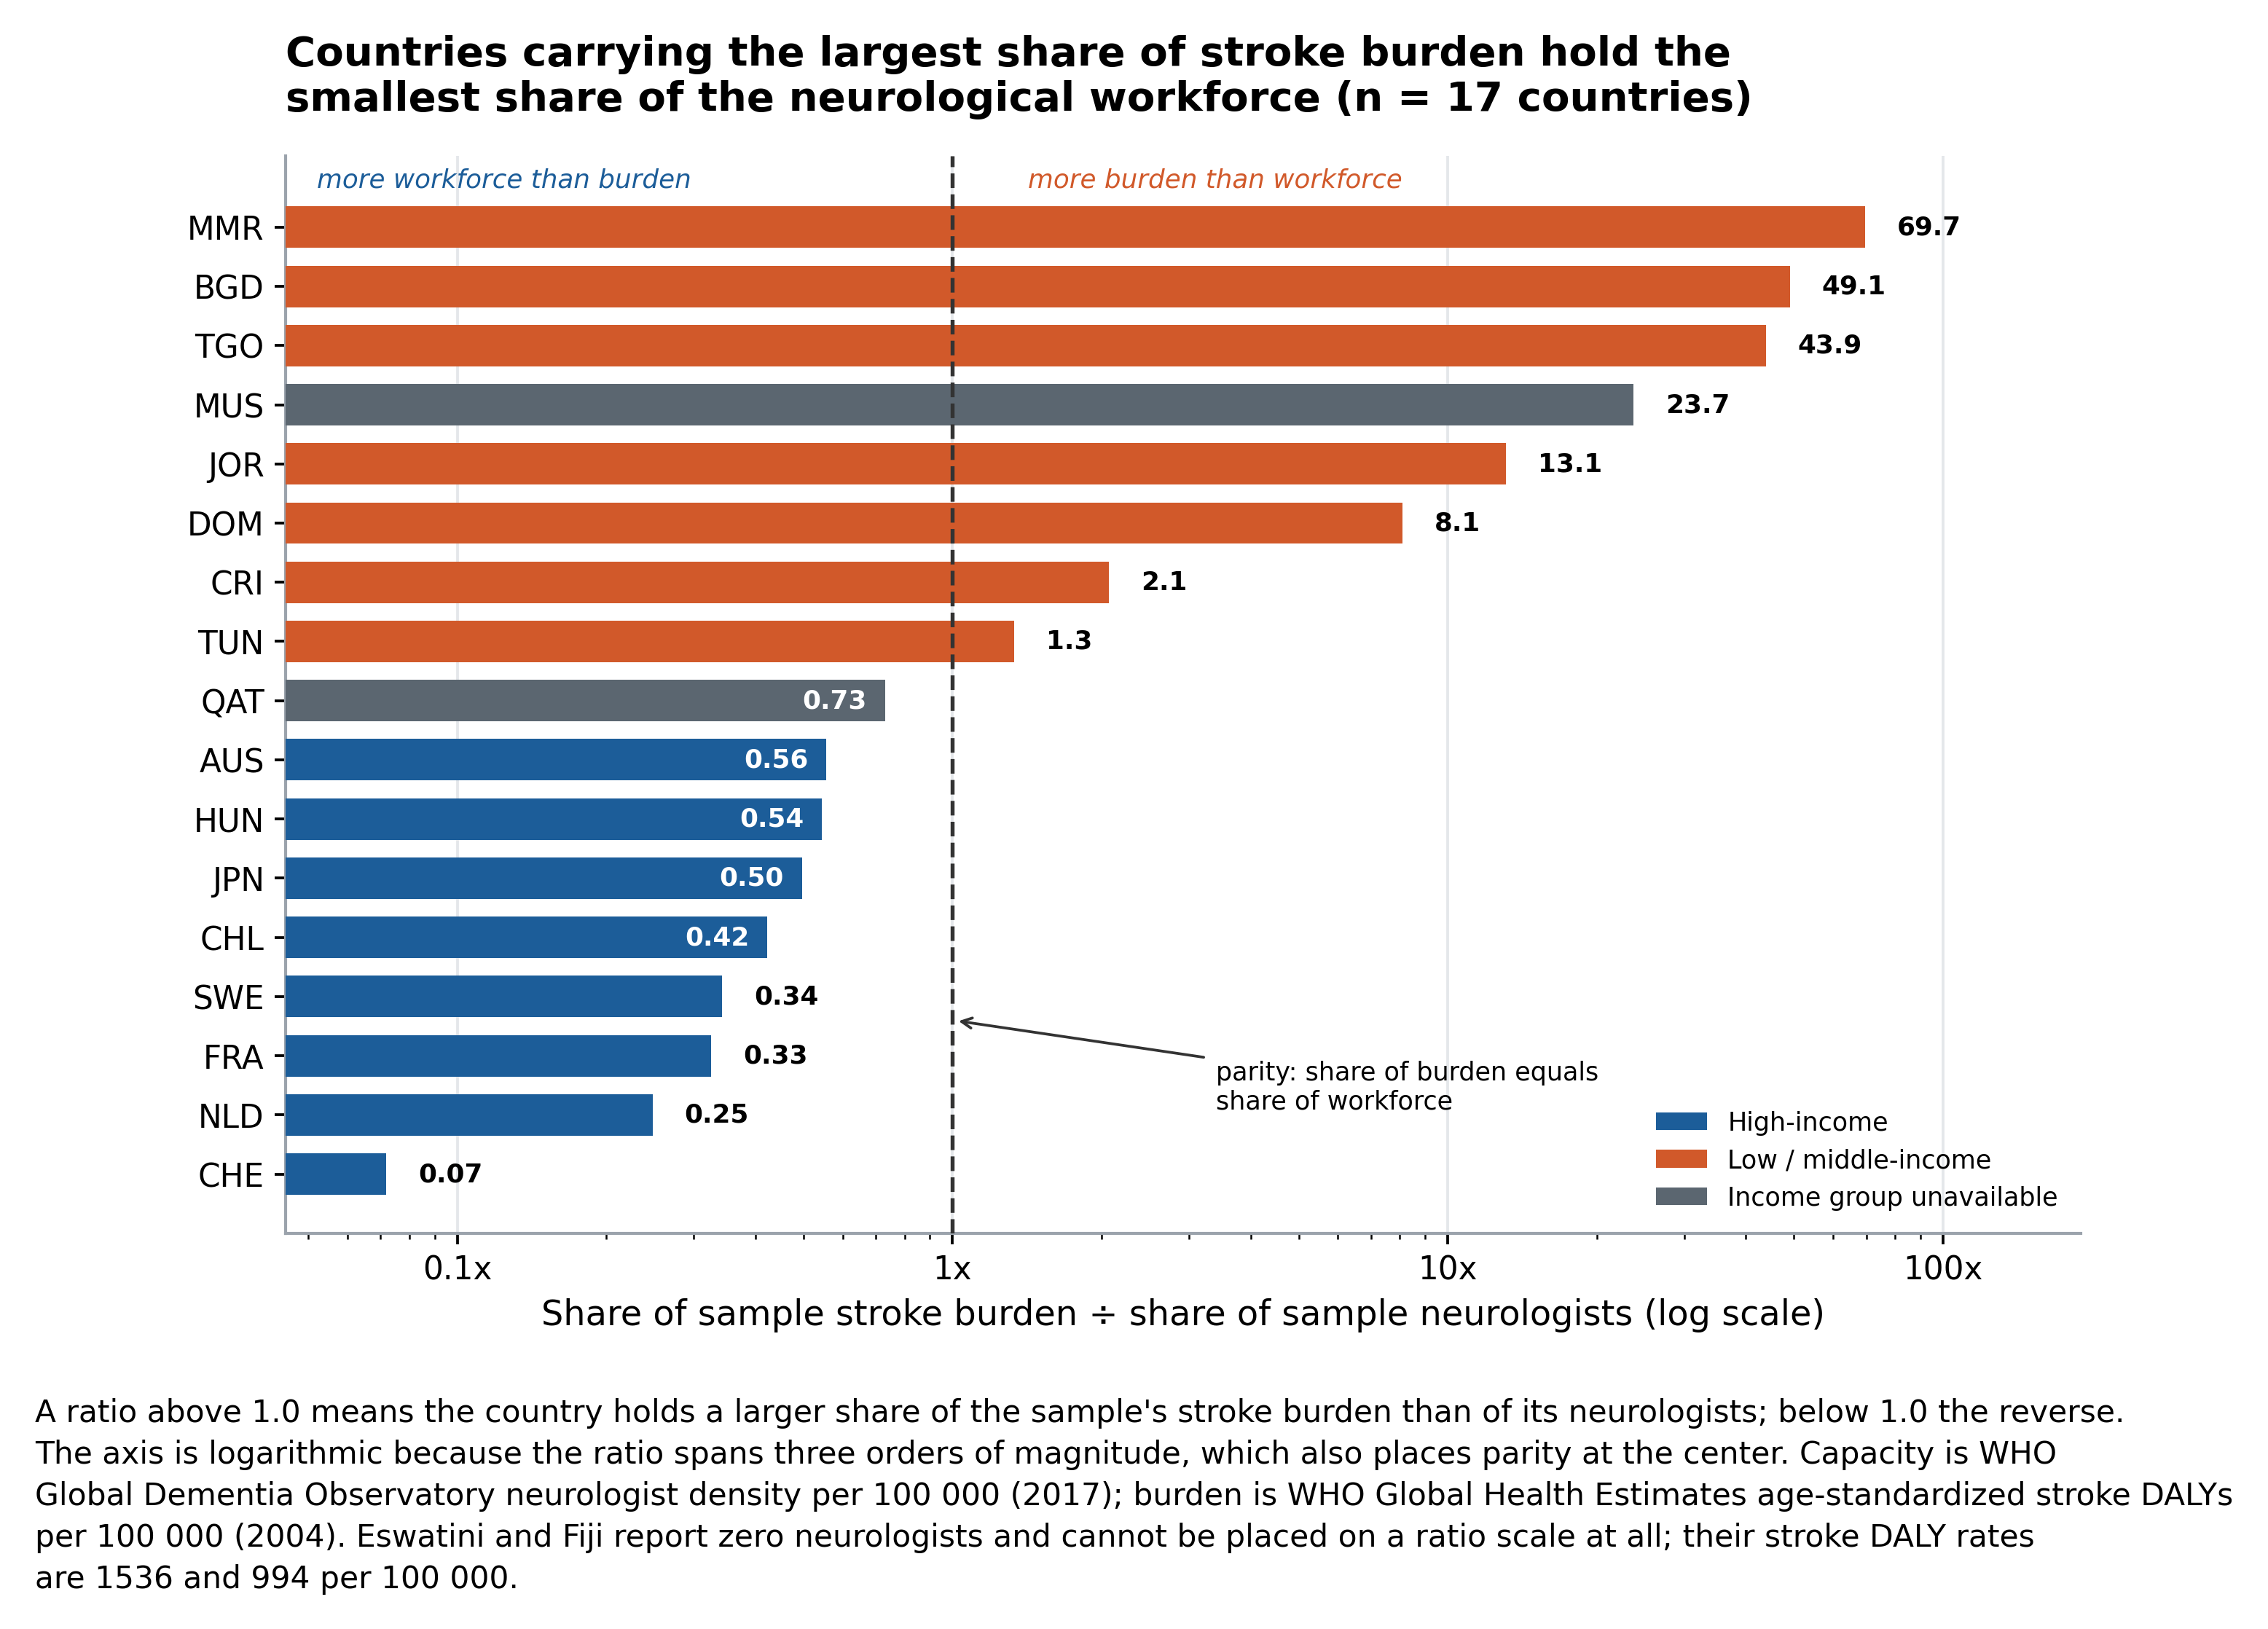
\includegraphics[width=0.74\linewidth]{figures/f01_alignment_ratio.png}
\caption{Burden-to-capacity share ratio by country, logarithmic axis. A ratio
above 1.0 means the country holds a larger share of the sample's stroke burden
than of its neurologists; below 1.0 the reverse. The axis is logarithmic because
the ratio spans three orders of magnitude, which also places parity at the
center. Capacity is WHO Global Dementia Observatory neurologist density per
100{,}000 (2017); burden is WHO Global Health Estimates age-standardized stroke
DALYs per 100{,}000 (2004). $n = 17$ countries placeable on the scale; Eswatini
and Fiji report zero neurologists and are excluded from the axis but discussed in
the text. Median high-income 0.38, median low/middle-income 13.12, a factor of
34.3.}
\label{fig:ratio}
\end{figure}

\subsection*{Capacity is distributed very unequally}

The Gini coefficient of neurologist density across the 19 reporting countries is
\textbf{0.61}, with a 95\% bootstrap interval of \textbf{[0.43, 0.73]}: high
inequality, imprecisely estimated. The poorer half of countries holds about
\textbf{6\%} of the sampled workforce. Inequality is greater between income
groups than within them, with a Gini of 0.27 within high-income countries and
0.49 within low- and middle-income countries. The focal contrast is Switzerland
at 13.10 per 100{,}000 against Myanmar at 0.07, a \textbf{187-fold} difference.
Dropping any single country moves the Gini by at most 0.06, so no one reporter
carries the result.

\begin{figure}%[tbhp]
\centering
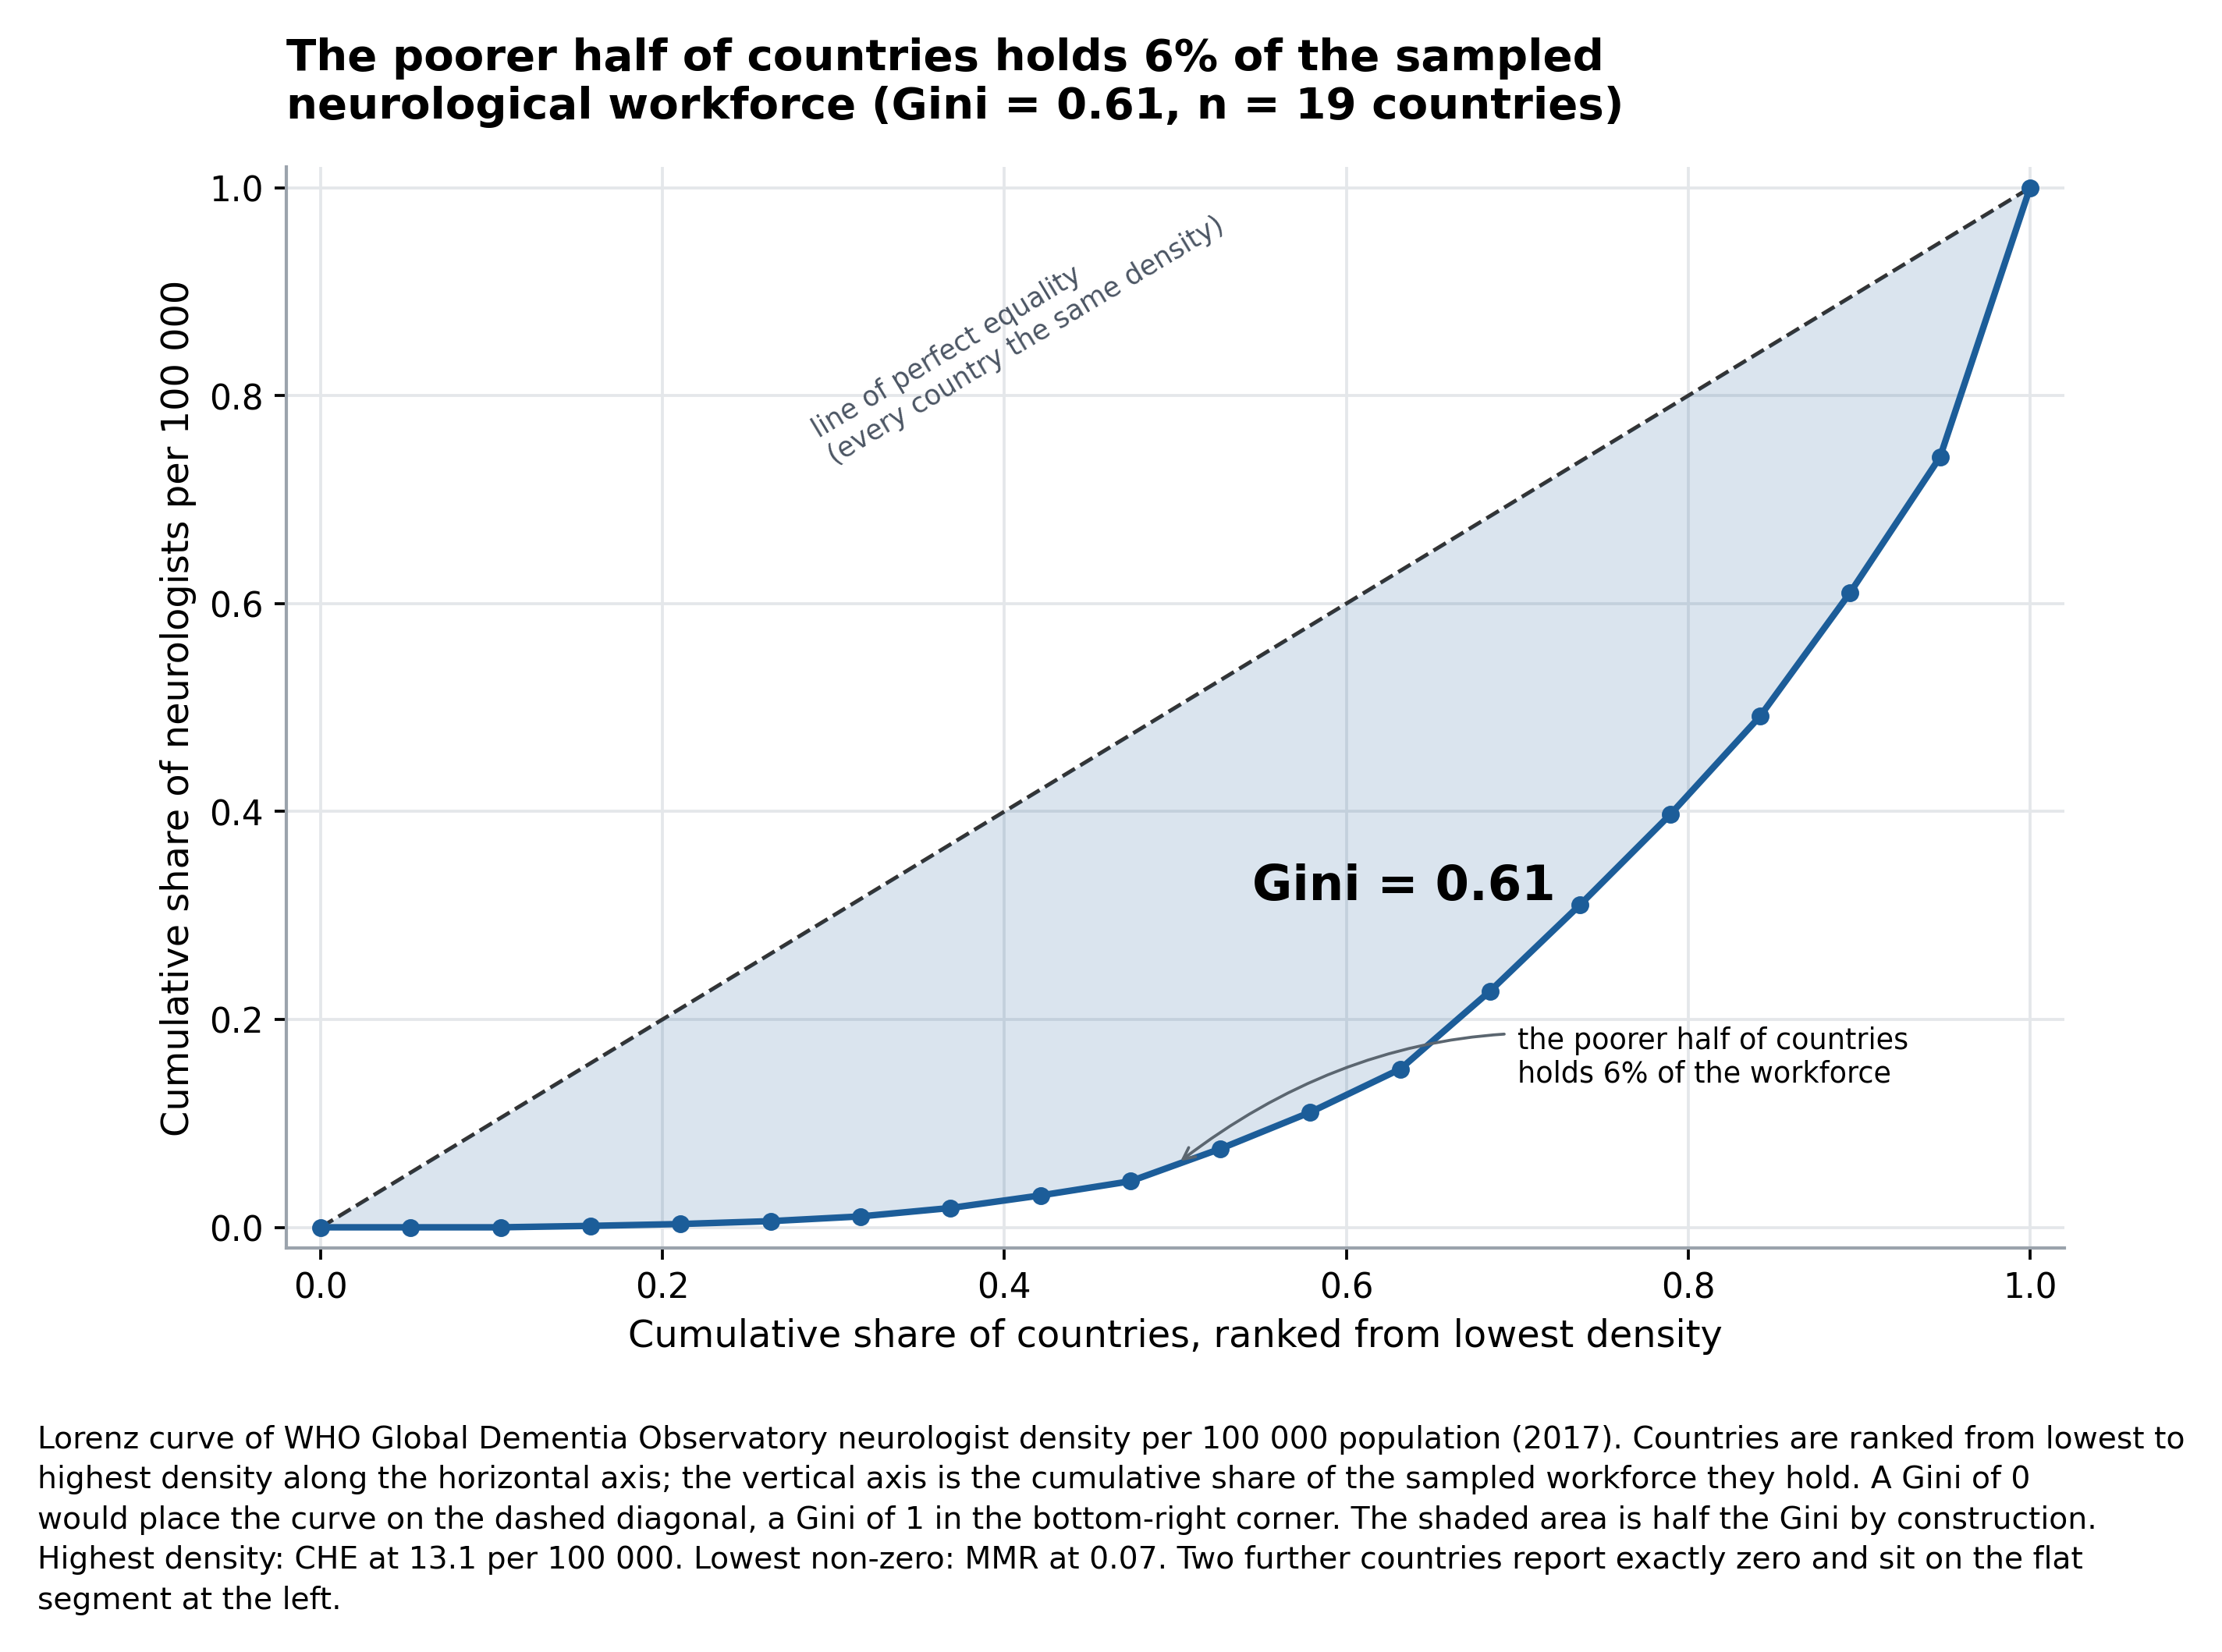
\includegraphics[width=0.74\linewidth]{figures/f02_lorenz_gini.png}
\caption{Lorenz curve of neurologist density across the 19 countries reporting a
workforce count. The horizontal axis is the cumulative share of countries,
ordered from lowest density to highest; the vertical axis is the cumulative
share of the sampled workforce they hold. Perfect equality would place the curve
on the diagonal, and the shaded area between the two is half the Gini
coefficient by construction. The poorest half of countries holds 6\% of the
workforce; the Gini is 0.61 (95\% bootstrap CI 0.43--0.73). Source: WHO/WFN
Neurology Atlas, 2nd edition (2017).}
\label{fig:lorenz}
\end{figure}

\subsection*{The gap differs systematically between country types}

Table~\ref{tab:tests} reports the binned comparisons. Neurologist density
differs between income bins on every test applied, including the
distribution-free permutation test. The most striking descriptive result is that
dementia diagnostic services reach rural areas in 77\% of high-income countries
and in \textbf{none} of the four low or lower-middle income countries sampled.

\begin{table}[t!]
\centering
\caption{Binned hypothesis tests. Country-level regressions are not fitted as
headline results because 19 to 35 observations cannot support them, so countries
are binned by World Bank income group and the groups compared directly. Rank-based
and permutation tests are reported alongside the parametric ones because the
chi-square has six of nine cells with expected counts below five.}
\label{tab:tests}
\begin{tabular}{llr}
\toprule
Comparison & Test & Result \\
\midrule
Density, high vs low/middle & Welch $t$ & $t = 4.29$, $P = 0.0031$ \\
\quad same & Mann-Whitney $U$ & $P = 0.0003$ \\
\quad same & Permutation (20{,}000) & $P = 0.0003$ \\
Reach across three bins & One-way ANOVA & $F = 5.74$, $P = 0.0074$ \\
\quad same & Kruskal-Wallis & $H = 9.44$, $P = 0.0089$ \\
Reach $\times$ income bin & Chi-square & $\chi^2 = 11.81$, $P = 0.0188$ \\
Rural reach $\sim$ high income & Logistic & OR $= 7.6$, $P = 0.0098$ \\
\bottomrule
\end{tabular}

\addtabletext{All tests are two-sided. The permutation test shuffles income-group
labels 20{,}000 times and assumes nothing about distributional shape.}
\end{table}

\subsection*{The gradient steepens with rarity}

Across the 114 Atlas respondents, the high-to-low income ratio is 71-fold for
total neurological workforce, 158-fold for adult neurologists, 62-fold for
neurosurgeons and \textbf{195-fold} for child neurologists. The scarcer the
cadre, the more concentrated it is in rich countries.

\subsection*{National density overstates access}

Figure~\ref{fig:urbanrural} reports both indices. UCI falls monotonically from
0.95 in low-income countries through 0.83 and 0.78 to 0.52 in high-income ones.
Effective rural density rises across the same groups from \textbf{exactly zero}
through 0.24 and 0.59 to 3.19 per 100{,}000. The zero is not
a rounding artifact: no low-income country in the Atlas reports a single
neurologist practicing rurally. The national gap between high- and low-income
countries is 71-fold; the rural gap has no denominator at all.



\begin{figure}%[tbhp]
\centering
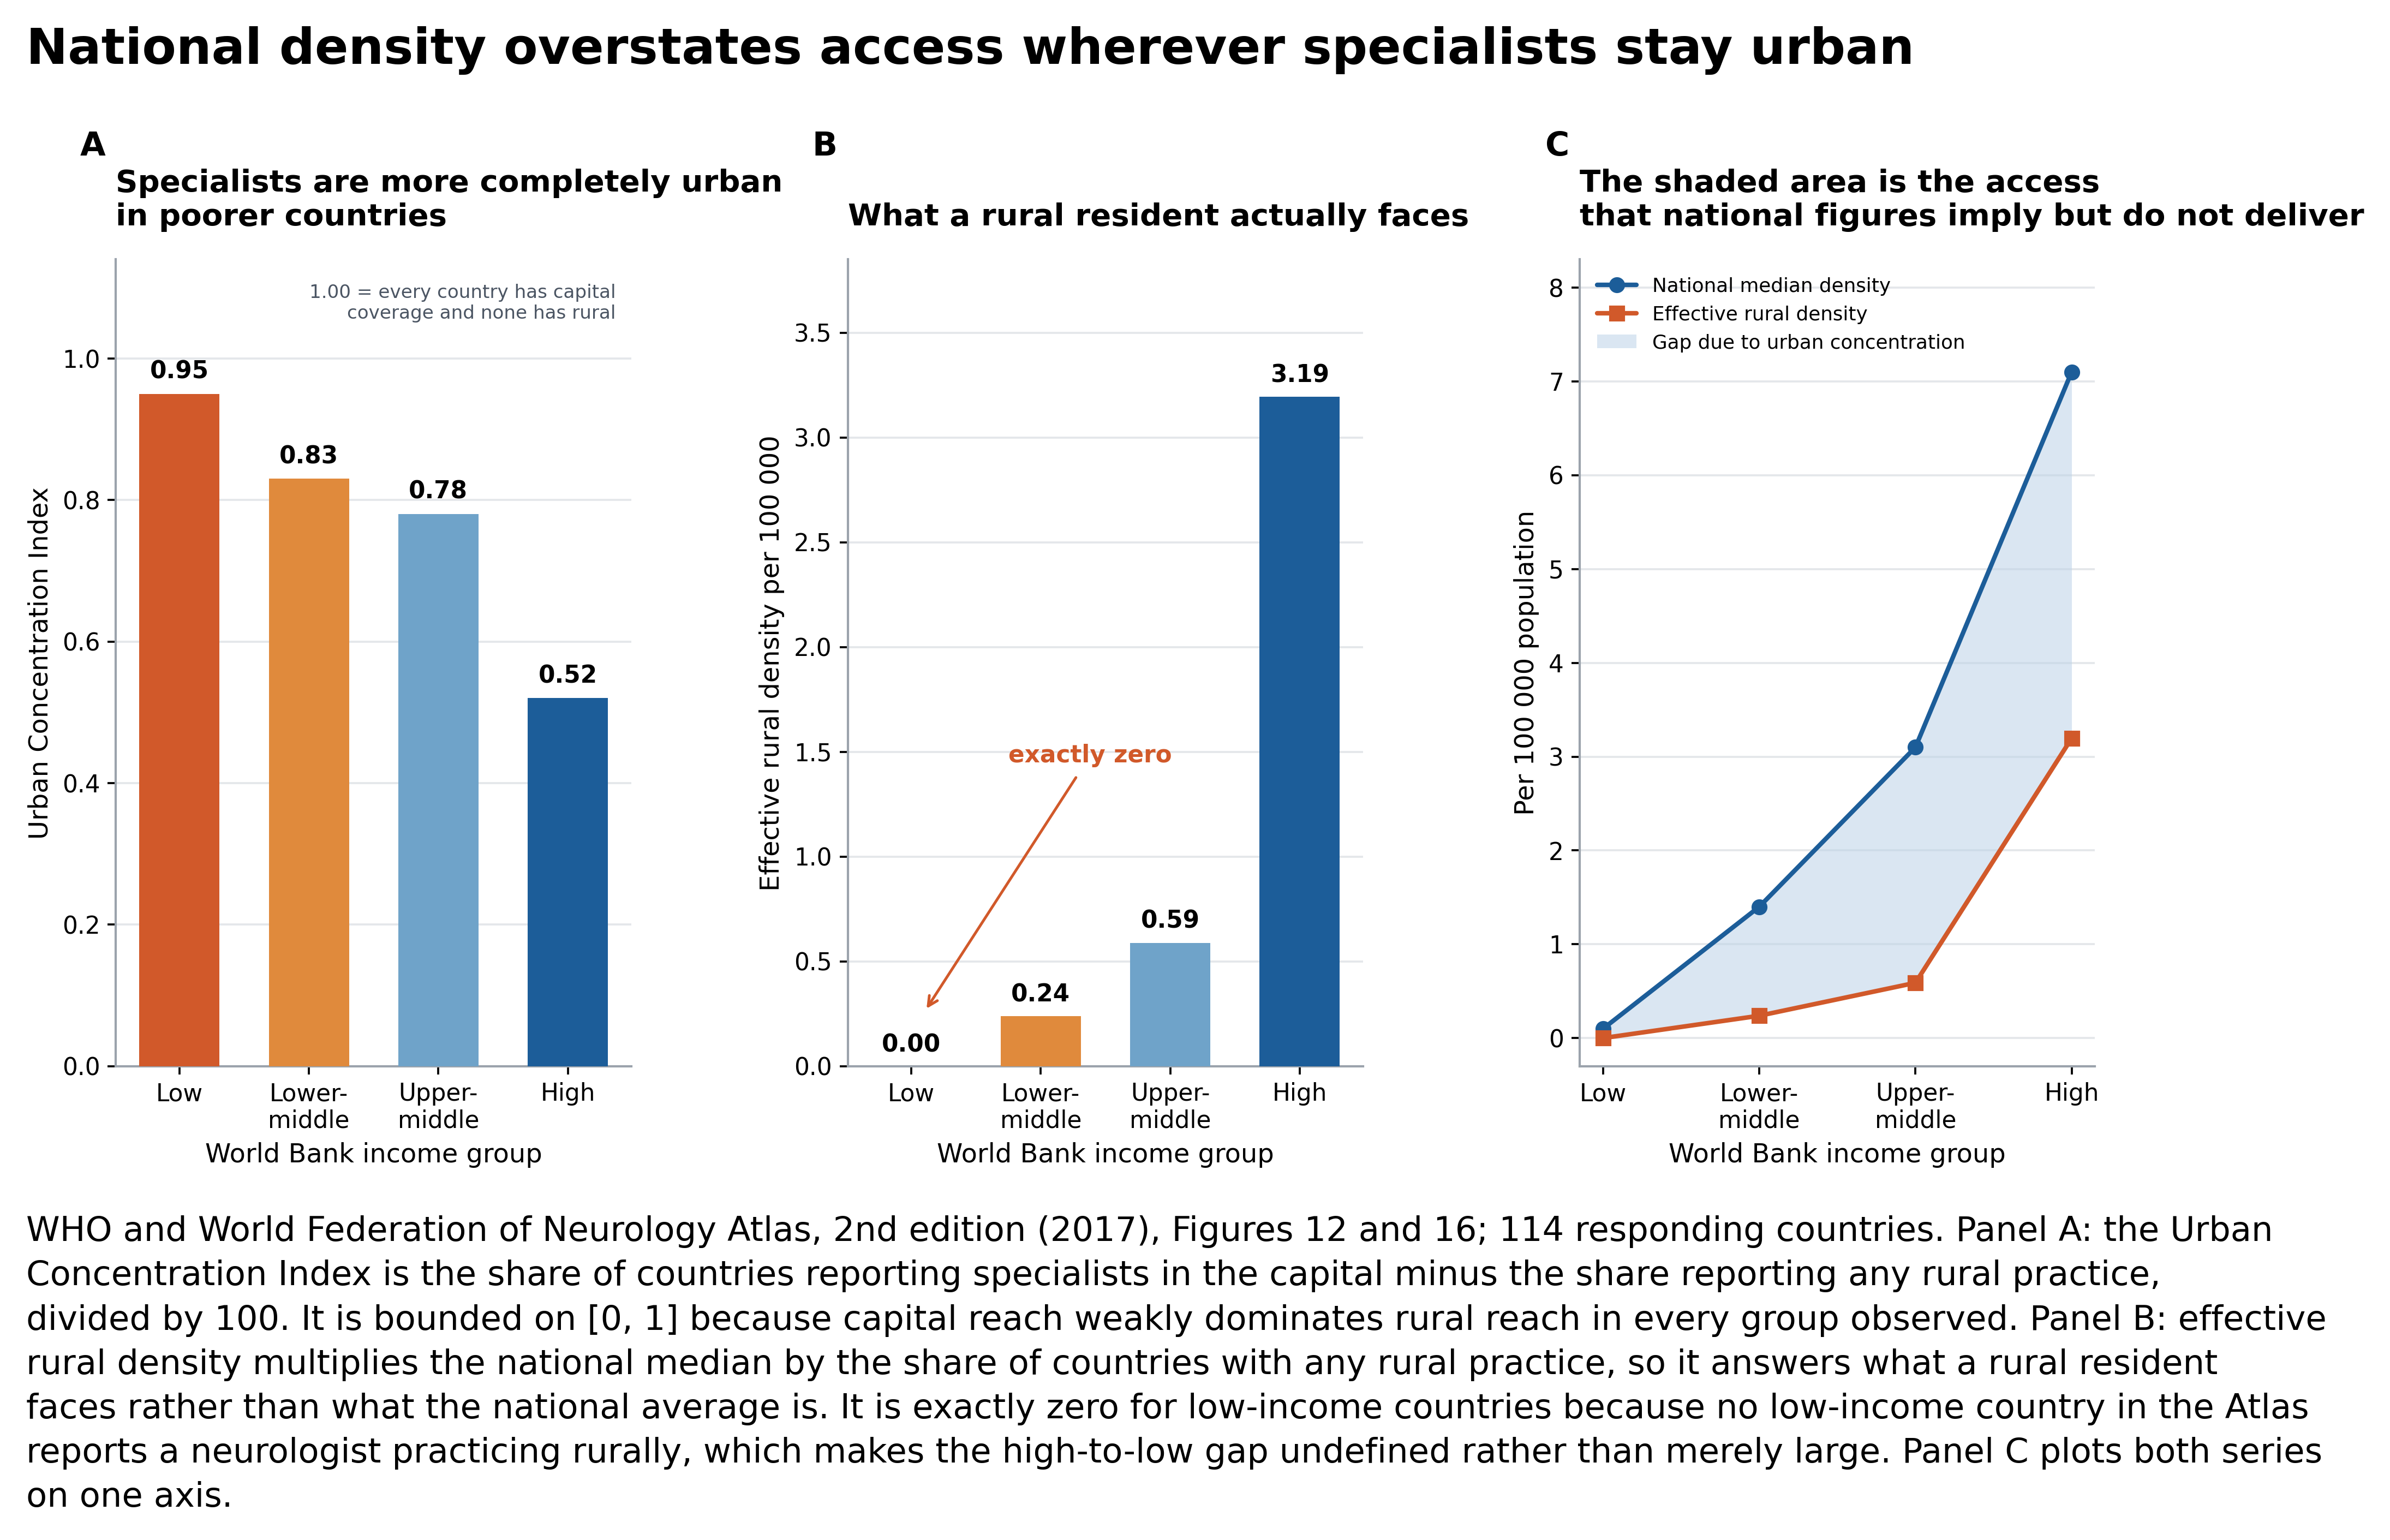
\includegraphics[width=0.74\linewidth]{figures/f06_urban_rural_indices.png}
\caption{National density overstates access wherever specialists stay urban.
Panel A: the Urban Concentration Index, the share of countries where
neurologists reach the capital minus the share where they reach rural areas.
Panel B: effective rural density, the national median rescaled by the share of
countries with any rural practice, which is the quantity a rural resident
actually faces. The low-income bar in Panel B is exactly zero, not rounded to
zero. Values by income group, low to high: UCI 0.95, 0.83, 0.78, 0.52;
effective rural density 0.00, 0.24, 0.59, 3.19 per 100{,}000. WHO/WFN Neurology
Atlas, 2nd edition (2017), 114 responding countries.}
\label{fig:urbanrural}
\end{figure}

\subsection*{An interaction the sample cannot resolve}

If capacity buys less alignment where services remain urban, capacity and rural
reach should interact. Only \textbf{13 countries} carry both measures. The
interaction coefficient is $-0.004$ with $P = 0.99$. That is a statement about
statistical power, not evidence that no interaction exists, and the figure title
in the repository says so explicitly rather than implying a null finding.

\subsection*{Robustness}

Three checks. A 5{,}000-draw bootstrap gives the Gini interval quoted above.
Leave-one-out moves the Gini by at most 0.06 for any single country. A bounding
exercise asks how much measurement error would be needed to overturn the central
result: burden in low- and middle-income countries would have to be
\textbf{overstated by a factor of 34}, or their capacity understated by the same
factor, for the two median ratios to level. Measurement error of that magnitude
is not plausible, and under-diagnosis in low-capacity settings pushes
\emph{measured} burden down rather than up, which widens the true gap rather
than closing it.

\section*{Discussion}

Across three metrics the finding is consistent: neurological capacity is
concentrated where measured burden is lightest, and national counts overstate
what most residents can reach. The policy implication is that specialists per
country is the wrong statistic for priority-setting. It answers a question about
supply when the operative question is about reach, and it is silent about
whether a rural resident can access anyone at all.

Six limitations bound the conclusion. The thirteen-year offset between capacity
and burden is the weakest joint. The samples are small and self-selected toward
countries with functioning health information systems, which understates the
gap. Stroke stands in for neurological burden generally. Six of nine cells in
the reach-by-income table have expected counts below five. Both WHO instruments
are self-reported and unaudited with no FTE adjustment. And the interaction test
is underpowered at 13 countries. Nothing here is a causal estimate.

Two extensions follow directly. The DHS inventory described in the repository
covers 106 countries and 443 surveys, 62 with GPS coordinates, which would
permit the same alignment question to be asked \emph{within} countries rather
than across them. And a burden series contemporaneous with the 2017 capacity
measures would remove the study's largest weakness.

\section*{Analyses not shown here}

Three figures and three tables appear above. The pipeline produces fourteen
figures and ten tables. The eleven figures held back are not weaker versions of
those shown; they answer adjacent questions, and each carries a self-contained
caption in the repository, numbered to match the script that writes it.

Four extend the descriptive picture: dementia service reach by income group,
Atlas workforce density across all 114 responding countries rather than the 19
with usable numbers, where inside a country neurologists practice, and the same
gradient split by clinical cadre. Two are geographic rather than economic,
showing capacity by WHO region with individual countries overlaid so
within-region spread stays visible. Three are paired instrument checks, placing
each Atlas aggregate beside its country-level counterpart from the Global
Dementia Observatory; two independently collected instruments ordering countries
the same way is weak evidence that neither is simply wrong. One reports DHS
survey and GPS coverage, which is groundwork for the subnational extension rather
than a result. The last compares the two regression solvers and verifies the
implementation rather than saying anything about neurologists.

The seven omitted tables hold the numbers behind results stated in prose above:
the Atlas gradients, the regression output, the interaction tests, the regional
comparison, the paired-instrument correlations, DHS coverage counts, and the
leave-one-out and bounding results.

\section*{Agentic Analysis}

I used Claude (Anthropic) as a coding assistant throughout. The transcripts are
in \texttt{docs/agentic/} in the repository. What follows is a reflection on
what I asked for, what I accepted, what I rejected, and where the assistant was
wrong.

\paragraph{What I asked for.} Scaffolding and implementation, not research
design. The research questions, the choice of a share ratio over a difference,
the decision to bin rather than regress, and the bounding exercise are mine. I
asked the assistant to implement estimators, restructure figure layout code, and
parse the Atlas PDF.

\paragraph{What I accepted.} The suggestion to implement the Gini twice, once by
the sorted-index formula and once by integrating under the Lorenz curve, as a
mutual check. The two agree to $1.1\times10^{-16}$. I accepted the same argument
for solving the normal equations alongside gradient descent. Both are cheap and
both would have caught a transcription error in the algebra.

\paragraph{What I rejected.} The assistant initially proposed fitting a
country-level regression of the alignment ratio on capacity and reporting the
slope as a headline result. On 19 observations that slope is not identified in
any useful sense, and reporting it would have implied precision the data cannot
support. I replaced it with binned comparisons and a permutation test. The
regression survives only as a solver check.

It also proposed dropping the countries reporting zero neurologists, because
they are undefined on a ratio scale and break the plot. Dropping them would have
removed the two most extreme cases of the phenomenon the paper is about.
They are reported separately instead.

\paragraph{Where the assistant went wrong.} Three failures, all of the same
shape.

First, a figure title. An earlier revision produced a panel titled ``adding
capacity does not help equally in every country,'' describing an interaction
whose coefficient was $-0.004$ at $P = 0.99$. The code ran, the figure rendered,
and the title asserted a finding the numbers did not support. It now reads ``the
interaction the 13-country sample cannot resolve, beside the comparison it
can.''

Second, silent truncation in the PDF parser. The Atlas Annex wraps two long
country names across lines, and the first parser took only the first line,
yielding ``The former Yugoslav Republic of'' as a country. A generalized fix
then over-corrected and glued contributor names onto countries. The rule that
worked keys on the fact that a wrapped country name is cut mid-phrase and ends
in a function word, which no contributor name does. Eight assertions against
values read off the page now guard the parse.

Third, a data exposure I did not ask about and was not warned of. The DHS
inventory the assistant built retained the authenticated download URLs in a
committed column. Those URLs are tied to my approved DHS account. The analysis
never needed them; \texttt{02\_build\_dhs\_inventory.py} now discards them at
parse time.

\paragraph{What this implies.} The common structure is fluent, well-commented
code producing output that is wrong in a way the code does not reveal. Writing
the code became fast; verifying that it answered the intended question became
the binding constraint. In all three cases the error surfaced only when I asked
what a quantity \emph{meant} rather than whether the script ran.

\section*{Materials and Methods}

All code, committed data and figures are at
\url{https://github.com/alannap27/qss20-neuro-access}, organized as numbered
scripts in \texttt{code/}, committed inputs in \texttt{data/}, and figures and
tables in \texttt{output/}. Shared functions are in \texttt{code/utils.py} and
figure layout rules in \texttt{code/figstyle.py}. No script contains a hardcoded
absolute path. The WHO inputs are public and committed; the Neurology Atlas PDF
and the DHS manifest are excluded, the first because it is a copyrighted
publication and the second because its URLs are tied to an approved DHS account.
Analyses used Python 3.10 with pandas, NumPy, SciPy, statsmodels and Matplotlib;
versions are pinned in \texttt{requirements.txt}. Random seeds are fixed
throughout.

\dataavail{Every figure and table in this paper, and the eleven figures and seven
tables not shown, are regenerated from the committed data by \texttt{bash
run\_all.sh}. The two scripts that rebuild \texttt{data/raw/} from restricted
sources are excluded from that command and print an explanation rather than
failing when their inputs are absent.}

\acknow{I thank Prof.\ Herbert Chang for guidance on the analysis design and for
the suggestion to bin countries rather than fit underpowered country-level
regressions.}

\showacknow % Display the acknowledgements section

% Bibliography
\bibliography{qss20}

\end{document}
